\documentclass[article,12pt,onesidea,4paper,english,brazil]{abntex2}

\usepackage{lmodern, indentfirst, nomencl, color, graphicx, microtype, lipsum}			
\usepackage[T1]{fontenc}		
\usepackage[utf8]{inputenc}		

\setlrmarginsandblock{2cm}{2cm}{*}
\setulmarginsandblock{2cm}{2cm}{*}
\checkandfixthelayout

\setlength{\parindent}{1.3cm}
\setlength{\parskip}{0.2cm}

\SingleSpacing

\begin{document}
	
	\selectlanguage{brazil}
	
	\frenchspacing 
	
	\begin{center}
		\LARGE ESTÁGIO DE MUDANÇA DE COMPORTAMENTO PARA REALIZAÇÃO DE ATIVIDADE FÍSICA1
		
		\normalsize
		 Maria Vitória Dunice Pereira\footnote{Aluna do Curso Técnico em Química Integrado ao Ensino Médio, mvitoriadunice@gmail.com,
			Campus Porto Velho Calama, membro do GESSTEC/IFRO.
		} 
		Iranira Geminiano Melo\footnote{Orientadora, iranira.melo@gmail.com, Campus Porto Velho Calama, membro do GESSTEC/IFRO.} 
		
	\end{center}
	
	% resumo em português
	\begin{resumoumacoluna}
	Conhecendo o estágio de mudança de comportamento para realização de atividade física em que se encontram os estudantes podem ser desenvolvidas estratégias de sensibilização para que eles possam melhorar o estágio visando o estágio de manutenção, contribuindo de forma positiva para a qualidade de vida. Assim, este estudo teve por objetivo estudar os estágios de mudança de comportamento para atividade física com alunos do ensino técnico integrado ao médio. Obtendo-se como resultado um questionário de pesquisa interativo.
		
		\vspace{\onelineskip}
		
		\noindent
		\textbf{Palavras-chave}:Saúde. Tecnologia. Hábitos.
	\end{resumoumacoluna}
	
	\section*{Introdução}
	
	A agitação do cotidiano é associada ao sedentarismo e as pessoas justificam seus maus hábitos com a falta de tempo, porém a mudança de algumas práticas podem resultar em uma melhoria satisfatória na saúde física e mental do indivíduo.
	
	A tecnologia surge para nos auxiliar em diversas situações de nossas vidas, uma delas em nossa saúde. Torna-se necessário conhecer o estágio de mudança  de comportamento para realização de atividade física, que pode ser de (do mais para o menos positivo): Estágio de manutenção (quando a pessoa se exercita regularmente há mais de seis meses), estágio de ação (a pessoa pratica atividades físicas regularmente a menos de seis meses), estágio de preparação (a pessoa não se exercita de forma regular, mas pretende fazê-lo nos próximos 30 dias), estágio de contemplação (a pessoa tem intenção de fazer exercícios, mas não imediatamente) e estágio de pré-contemplação (a pessoa não pretende fazerexercícios).
	
	\section*{Material e Método}
	
Esta é uma pesquisa qualitativa desenvolvida a partir da informatização de um formulário, utilizando-se as linguagens PHP, CSS, Java Script, HTML e SQL e desenvolveu-se um banco de dados para armazenar os resultados dapesquisa.

O questionário informatizado tem por título Estágio de Mudança de Comportamento - Atividade Física de Nahas (2013). Ao acessar o site o participante da pesquisa encontrará o seguinte questionamento: “Você tem um estilo de vida fisicamente ativo?”, caso a alternativa selecionada pelo aluno seja negativa, aparecerá a pergunta “Você considera a atividade física importante para a sua  saúde e bem-estar em geral?”, logo em sequência, caso positiva segue a questão “Você pratica há mais de seis meses?” finalizando o questionário. Caso o participante responda sim à primeira questão aparecerá a pergunta “Você pratica há mais de seis meses?”, e se encerra o questionário aparecedo o resultado do teste.
	
	\section*{Resultados e Discussão}
	
	Na pesquisa teve-se como resutado um site onde está hospedado o questionário conforme figuras 1 e 2. Na figura 1 está uma representação do questionário que está hospedado no site do Grupo de Estudos Saúde, Sociedade e Tecnologia.
	\begin{figure}[h]
		\centering
		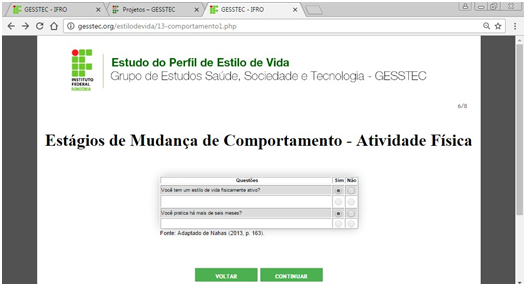
\includegraphics[width=0.7\linewidth]{pip-pg75-01}
		\caption{Ilustração do questionário.}
		\label{fig:pip-pg75-01}
	\end{figure}

	Na figura 2 tem-se uma ilustração do resultado que é apresentado ao participante da pesquisa. No caso, representando um estágio de ação com o anime mostrando felicidade, por ser o melhor estágio.
	\begin{figure}[h]
		\centering
		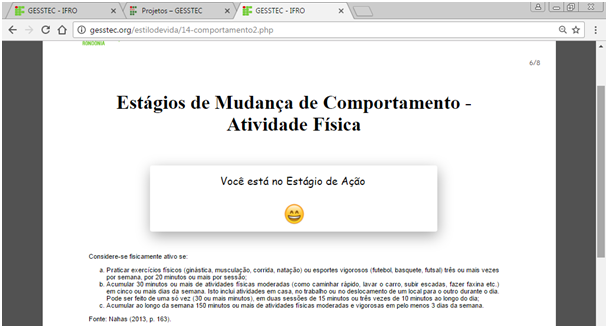
\includegraphics[width=0.7\linewidth]{pip-pg75-02}
		\caption{Ilustração de resultado, Porto Velho, 2016.}
		\label{fig:pip-pg75-02}
	\end{figure}
	
	
	\section*{Conclusões}
	
	Nesta pesquisa a tecnologia foi aproveitada com a intenção de melhorar a coleta de dados e fornecer resultado imediato ao participante da pesquisa sensibilizando-o para adoção de um estilo de vida ativo.
	
	
	\section*{Referências}
	
	\noindent NAHAS, Markus V. Atividade física, saúde e qualidade de vida. 6. ed. Londrina: Midiograf,2013.
	
\end{document}